\chapter{System Design}
\label{chapter:design}

\section{Overview}
The architecture of our system is shown in Figure~\ref{fig:system_architecture}. The Ethrerum blockchain
\begin{figure}[hb]
    \centering
    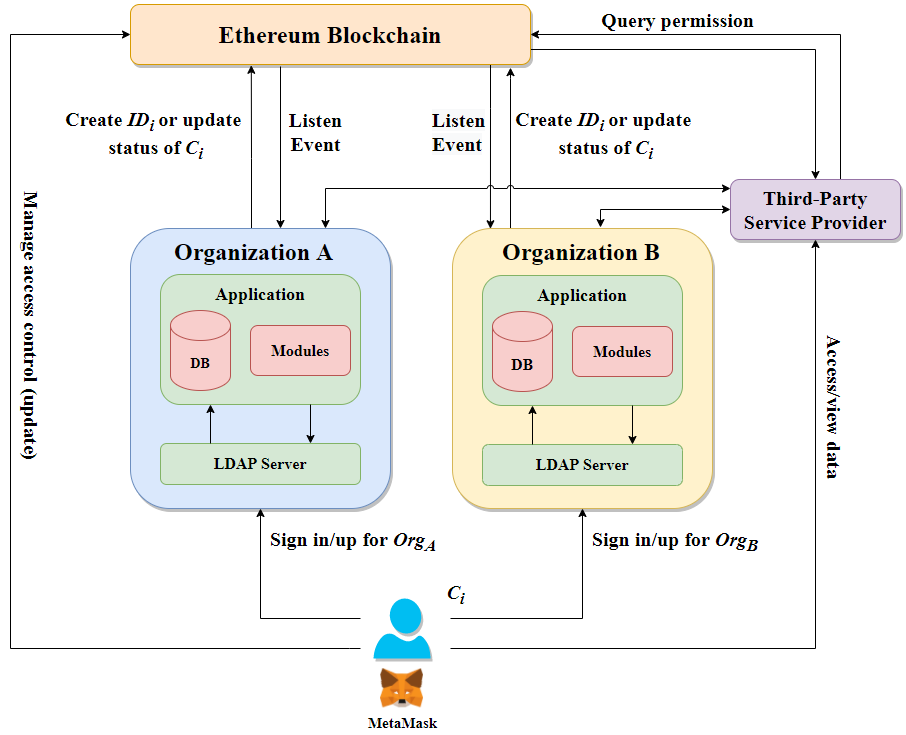
\includegraphics[height=!,width=1\linewidth,keepaspectratio=true]{figures/system_architecture.png}
    \caption{{\footnotesize System Architecture}}
    \label{fig:system_architecture}
\end{figure}

\newpage
\begin{figure}[hb]
    \centering
    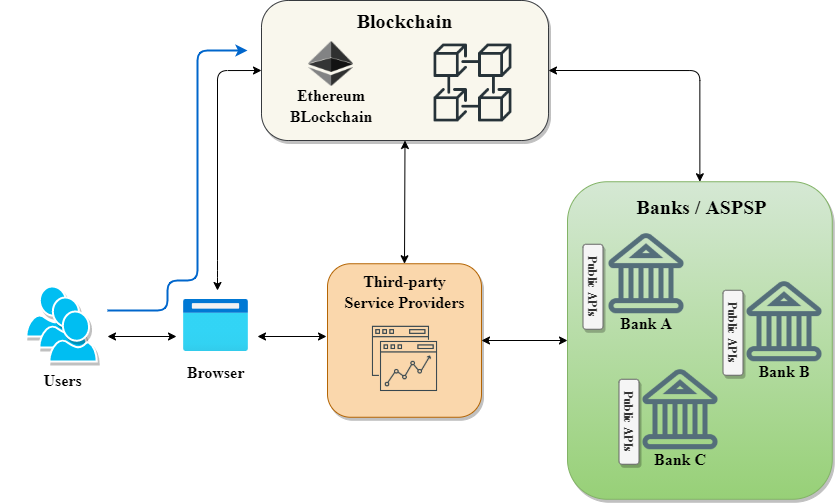
\includegraphics[height=!,width=1\linewidth,keepaspectratio=true]{figures/system architecture-banks.png}
    \caption{{\footnotesize Relation between open banking roles}}
    \label{fig:relation}
\end{figure}
    In order to apply our proposed system to open banking ecosystem, we have three clearly defined roles: Customer (User), Financial institution, and Third-party services provider. Figure~\ref{fig:relation} gives an overview of our proposed system. It shows the relation between these roles and includes workflows, detailed in Sect.~\ref{ssec:workflow} Each customer interacts with Blockchain by using MetaMask, they not only login with MetaMask but also manage their own access manager contract. That's why customers can allow the specific party to access their data.

\section{Scenario}

    For user perspective, our proposed system provide a single digital ID with Ethereum blockchain.

\section{Workflow} \label{ssec:workflow}
\begin{itemize}
    \item Verify unique ID stage
    \item Binding account stage
    \item Third party login stage
\end{itemize}
\subsection{Identity verification}
\subsection{Account binding}
\subsection{Third-party login with Ethereum account}
\subsection{Data sharing}